%%%%%%%%%%%%%%%%%%%%%%%%%%%%%%%%%%%%%%%%%%%%%%%%%%%%%%%%% 
% Following block written by Ziwen Fu 
%%%%%%%%%%%%%%%%%%%%%%%%%%%%%%%%%%%%%%%%%%%%%%%%%%%%%%%%%

\documentclass[amsfonts, showkeys, tightenlines,aps,12pt,floatfix]{revtex4}
% showpacs
\usepackage{bm}
\usepackage{epsfig}
\usepackage{graphicx}
\setlength{\oddsidemargin}{0in}
\setlength{\evensidemargin}{0in}
\setlength{\textwidth}{6.25in}
\setlength{\topmargin}{-0.1in}
\setlength{\textheight}{9in}

%%%%%%%%%%%%%%%
% You should use BibTeX and apsrev.bst for references
% Choosing a journal automatically selects the correct APS BibTeX style file 
% (bst file), so only uncomment the line below if necessary.
\bibliographystyle{apsrev}

\begin{document}

% Use the \preprint command to place your local institutional report
% number in the upper righthand corner of the title page in preprint mode.
% Multiple \preprint commands are allowed.
% Use the 'preprintnumbers' class option to override journal defaults
% to display numbers if necessary
%\preprint{}

%Title of paper
\title{Snobfit on Reflectometry }
\author{Ziwen Fu}
\email{fzww@yahoo.com.cn}
\author{P.~A.~Kienzle}
\email{paul.kienzle@nist.gov}
%\homepage[]{Your web page}
\thanks{}

\affiliation{University of Maryland/
             National Institute of Standards and Technology
}

% Date
\date{\today}

\begin{abstract}
We revisit snobfit (Stable Noisy Optimization by Branch and Fit), 
reimplementing the algorithm in the Python programming language, 
incorporating the statistical analysis of the fitting parameters,
making it work on high dimensional problems (e.g., $n>10$ ), and
testing it on a new class of test functions for global optimization.
We demonstrate this enhanced version on fits to experimental data
from neutron and X-ray reflectometry.

% insert suggested PACS numbers
%\pacs{}

%==================================================================
% insert suggested keywords - APS authors don't need to do this
\keywords{ Python, Global optimization, Constrained, Algorithms, 
           branch and bound, derivative-free, surrogate model, 
           parallel evaluation, hidden constraints
}

\end{abstract}

%\maketitle must follow title, authors, abstract, \pacs, and \keywords
\maketitle

\section{\label{intro}Introduction}
Snobfit~\cite{Neumaier} is a global optimizer which uses a 
surrogate-based strategy to model the response surface. It builds 
local quadratic models from the suggested evalution points and 
performs a global search over these models by branching and local 
fits.  It is specicially designed for expensive objective functions 
where some noise can be present. 

Neutron reflectometry analysis is an inverse problem with many
closely spaced local minima.  The magnitude of the reflection
quickly decreases with angle, leading to increasingly
noisy signals as reflection angle increases.  
The reflectivity calculation can be moderately expensive 
(about 1~s for 1-D models, up to 250~s for 3-D models). 
Analytic derivatives are not readily available.  
When reflectometry is used to refine parameters for 
molecular dynamics simulations, calculation times will be better 
measured in days on high performance computers.  
These traits led us to assess Snobfit for our problems.

Snobfit is an expensive procedure suitable for low dimensional problems.
The existing Matlab implementation is used primarily ($n<10$)~\cite{Neumaier}.
For reflectometry, we need to be able to support medium scale problems, 
with dimension $n$ up to 200. Another potential issue is the number of local
minima in our fit space.  We needed to carefully assess the
performance of Snobfit on highly non-convex models.

In our role of providing support software for a national user
facility we need to reduce the burden on the user.  
To remove the requirement of a proprietary development environment, 
we have reimplemented Snobfit in Python.  Python~\cite{Python} is 
a freely redistributable general purpose dynamic object-oriented 
programming language.  In addition to support for numerical 
programming which rivals that of specialized environments such 
as Matlab, Python supports development and deployment of
native graphical user interface applications on multiple platforms
and has excellent support for network programming.  
It functions well as a glue language, with packages for connecting
to C, C++, Fortran, IDL and other environments of interest to
the scientific programming community.  Support amongst the
bioscience community is particularly strong.  The language is
well supported on the common user platforms of today (Windows and
Mac OS X) as well as server platforms (Linux/Unix) common on the grid.
The Python implementation of Snobfit performs significantly better
than the orginal Matlab implementation.

\section{\label{sec2} The Snobfit Algorithm}
The original Snobfit~\cite{Neumaier} is a Matlab 6 package 
for the robust and fast solution of noisy optimization problems
which supports bounds constraints and soft equality and inequality
constraints.~\cite{Dallwig}  Unfeasible points within the constrained
region are properly rejected.

?? What guarantees do we have about finding the global minimum?
e.g., Lipschitz?  What values of slope L?  Size of the acceptance
region?  Are there bounds on the number of evaluations given particular
properties of the function, such as number of minima or size of the 
acceptance rregions or height of the barriers?

Snobfit uses a branching strategy to search for the global minimum,
with a well behaved sequential quadratic programming method as the
local search.  Soft constraints are supported by a penalty-type method 
with nice theoretical properties.~\cite{Dallwig}  The fit can be
driven by hand, with each run of the program determining the next
set of parameters to be tested, or the software can drive the fit,
continually selecting new parameter sets until the global minimum is achieved.
Parameter sets are given in batches, which allows for easy small scale 
parallel function evaluations.\cite{Neumaier}

?? How much can we parallelize the next-points function?

The Python implementation of the Snobfit algorithm was 
developed by the reflectometry group at NIST 
(National Institute of Standards and Technology) and 
the University of Maryland.  This version supports the original Snobfit style
interface as well as providing new features:

\begin{itemize}
\item
An object-oriented interface, which allows many styles of
interaction with the underlying fit engine.  For example,
it is possible to call the new Snobfit without writing an
intermediate datafile storing the state of the fit each cycle.

\item
A functional interface, which allows the user to pass the
function to be optimized as a parameter to the fit.

\item
Statistical analysis of the results, returning uncertainty for
the optimized parameter values.

\item
Support for medium scale problems, up to at least $n=100$.

\item
Freely redistributable implementation which works on multiple computer
platforms (OS X, Linux, Windows).  Many thanks to the original Snobfit
authors for licensing their code with a BSD style license.  There are
few non-stochastic optimizers freely available to the scientific
programming community.

\item
Some changes to the branching algorithm which improve the performance
of the global search.

?? Can you quantify the improvement?  Or is it merely theoretically better?
Do you describe the improvement in this paper?

\end{itemize}

In the process of converting the code into Python and checking performance
on multiple platforms, we developed automated build and test tools for
the package.  This package will be included in an upcoming release of
SciPy, the common Python toolbox for scientific programming.

?? Make sure snobfit is in SciPy before removing this sentence!


\section{\label{sec3} Snobfit for Practical Global Optimization}
In Ref.~\cite{testClasses}, the authors describe a class of test functions 
which reflect a variety of difficulties encountered when solving 
practical optimization problems.   This test class has properties
similar to the reflectometry inverse problem.
Fig.~\ref{figure1} displays the two-dimensional test function
defined by Eq.~(6) in the above reference.  
We randomly chose an orthonormal matrix $\bf{A}$, yielding a function $F$
with a single global minimum at ${\bf{x^*}} = (0.51722532, 4.2109949)$
and $F({\bf{x^*}})=2$.  
Python Snobfit returned a minimum at ${\bf{x^*}} = (0.5172, 4.211)$,
with $F({\bf{x^*}})=2.00000013237$.  

\begin{figure}
\begin{minipage}[b]{0.8\linewidth}
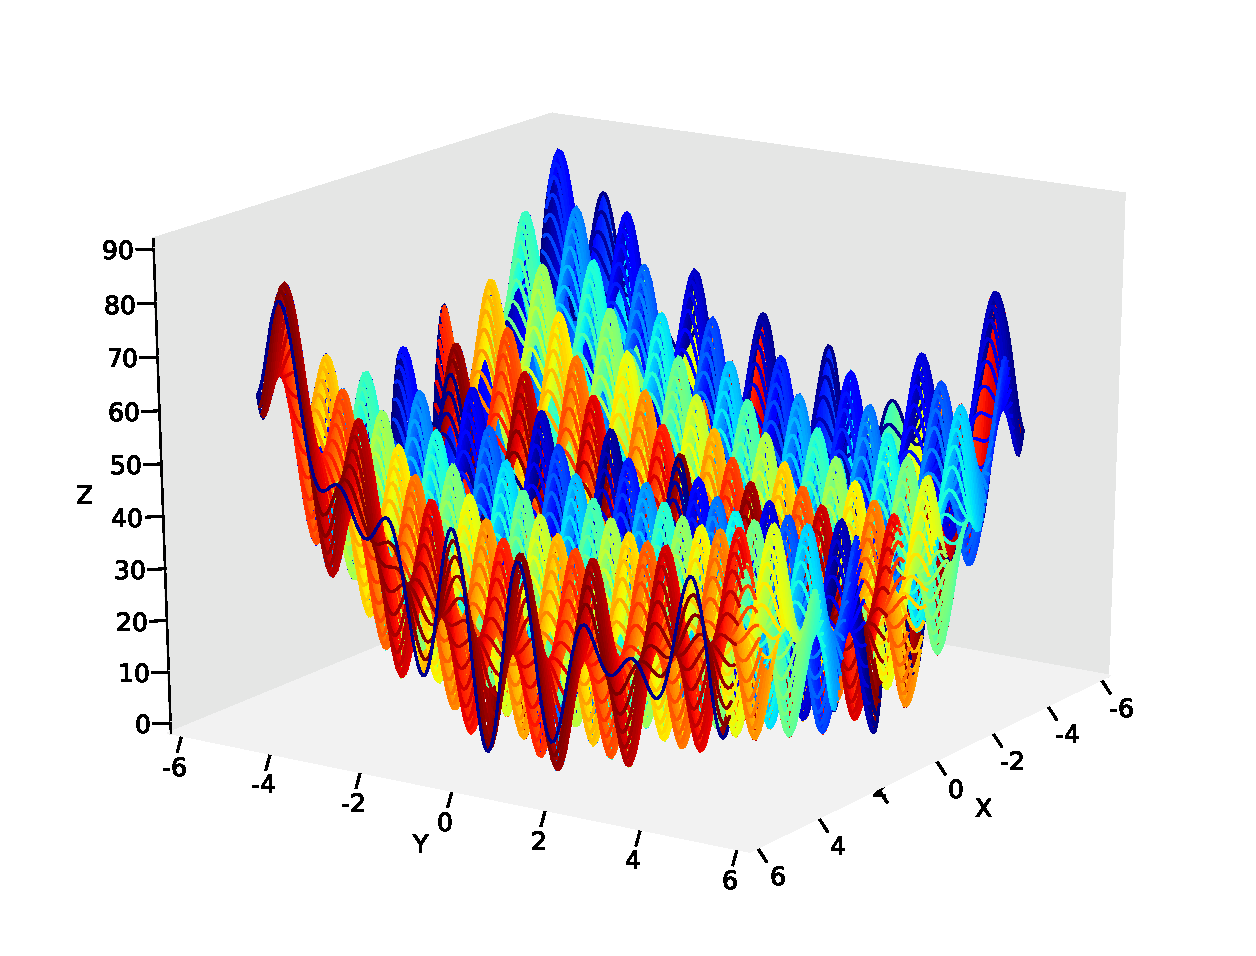
\includegraphics[width=1.0\textwidth]{testGO}
  \caption{A two-dimension function with $n=2, m=1,L2=2, L3=1, K=H=10, p=1, c1=-3$, and $c2=3$, over the box $[-5, 5]^2$. }
  \label{figure1}
\end{minipage}
\end{figure}

?? Differential Evolution~\cite{PriceStorn} failed to find the global 
minimum for this problem with a variety of choices for the algorithm
control parameters.  ??? To what extent did you vary the stochastic
component so that it was less prone to fall into a local minimum?
What is the number of evaluations required to get the correct solution
in DE 95\% of the time as compared to Snobfit?

?? Did you try any higher dimensional versions of this test problem, such as
$n=16$?  Are you convinced this problem is multimodal in higher dimensions?
Did DE work well in higher dimensions?

?? No mention of test of performance with noise, which I know you did
outside the context of reflectivity.

\section{\label{sec4} Snobfit and Reflectometry}
In this section, we show two applications to reflectometry, one
with dimension 2 and a second with dimension 20.

\begin{figure}
\begin{minipage}[b]{0.7\linewidth}
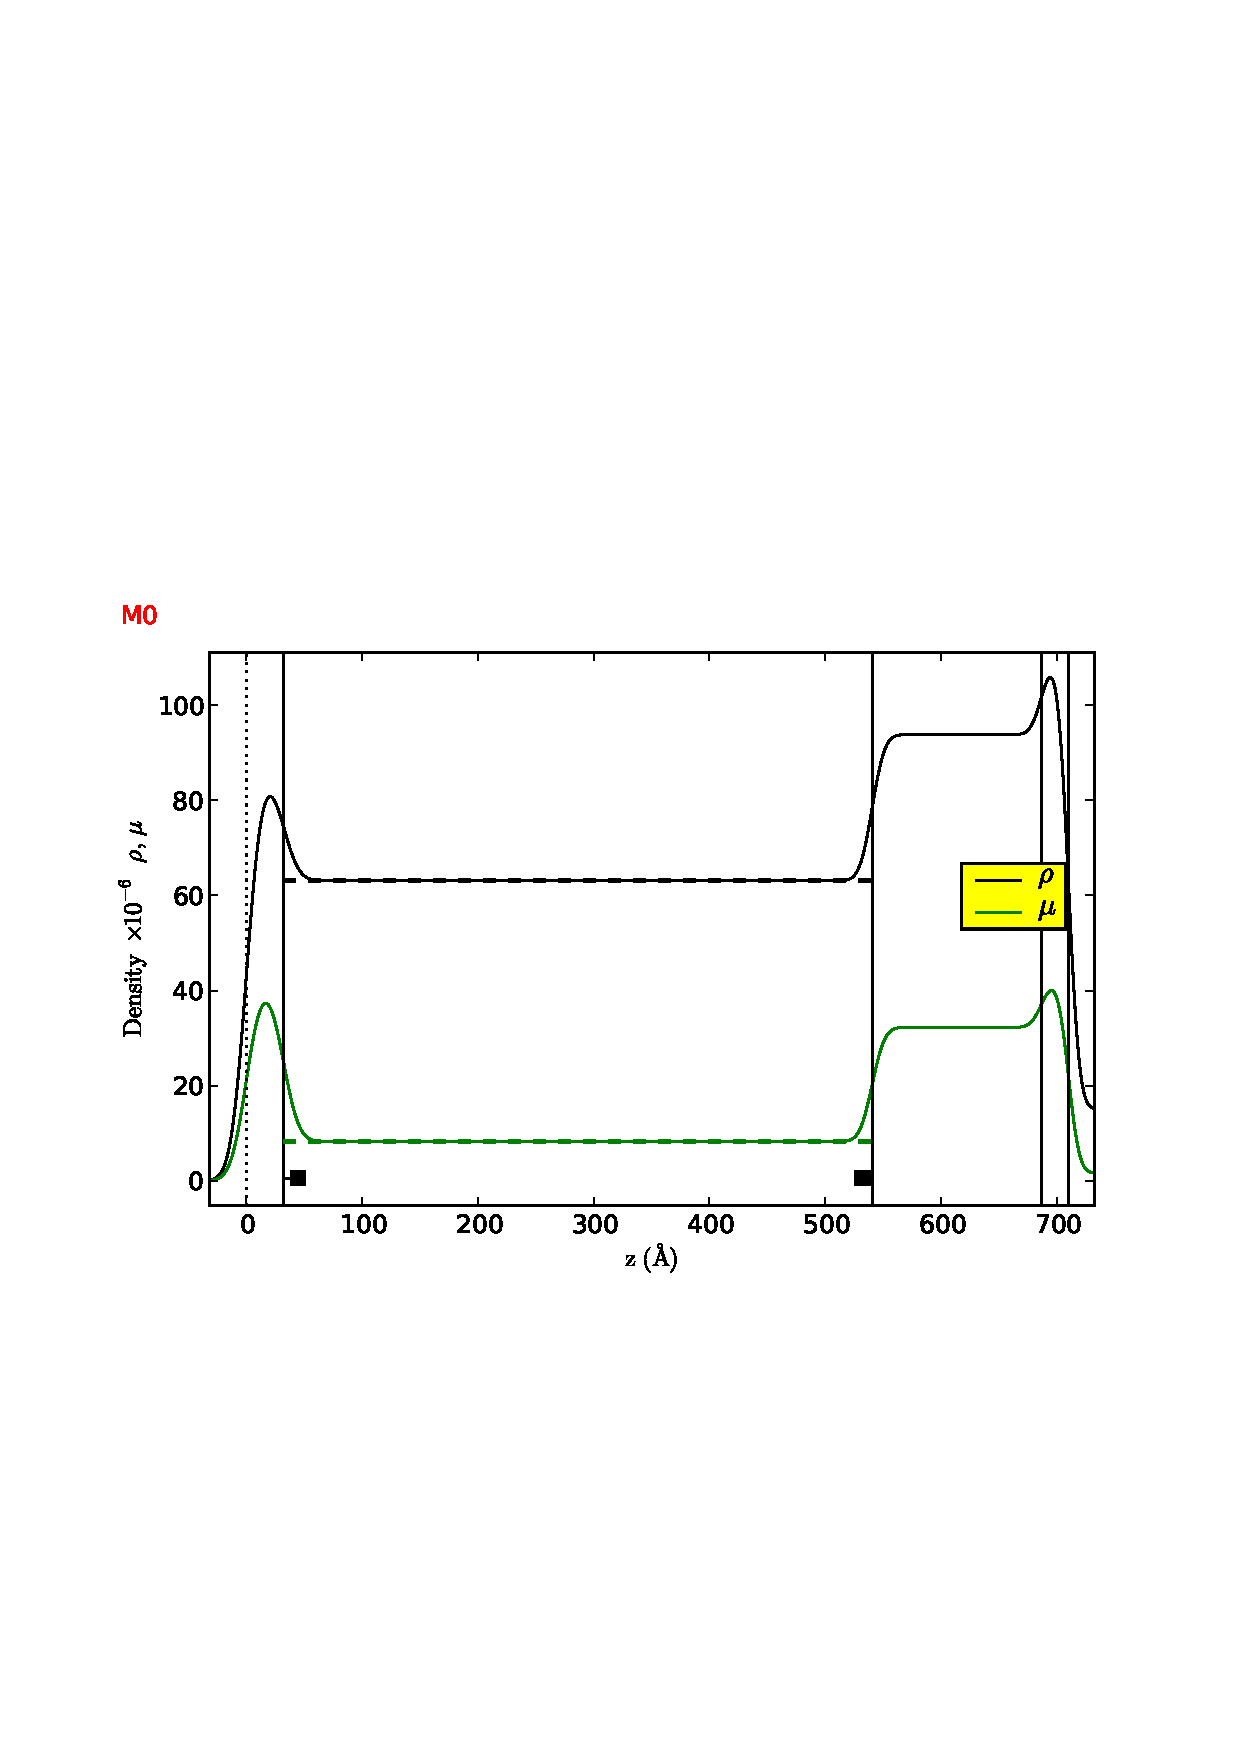
\includegraphics[width=1.0\textwidth]{profile}
  \caption{Density profile, measured data and best fit for a reflectivity
           experiment with ???sample descripton.}
  \label{figure2}
\end{minipage}
\end{figure}

\begin{figure}
\begin{minipage}[b]{0.7\linewidth}
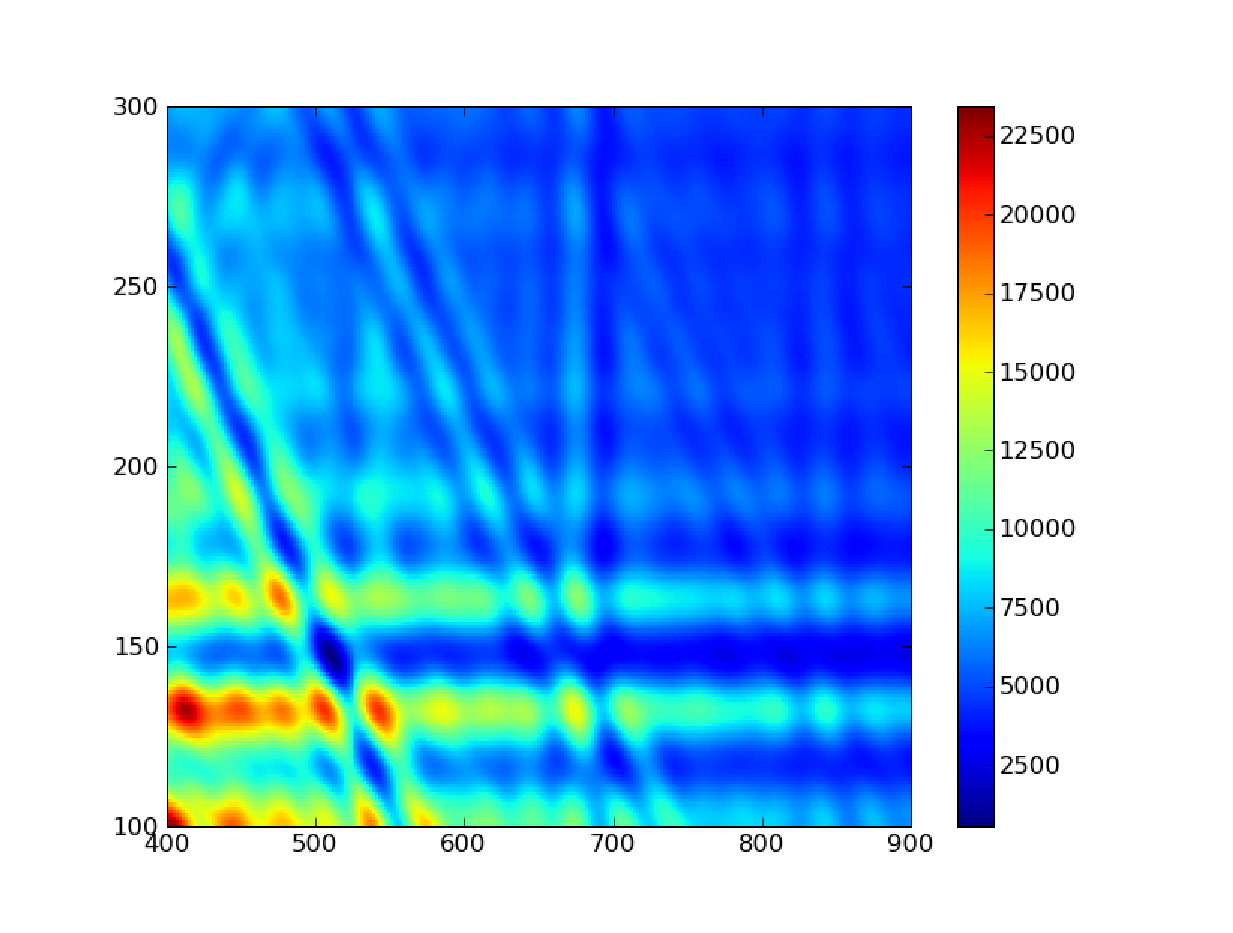
\includegraphics[width=1.0\textwidth]{chisq}
  \caption{Chisq plot for depth 2 x depth 3}
  \label{figure3}
\end{minipage}
\end{figure}

In Fig.~\ref{figure2}, we show the profile of the reflectometry problem.
In Fig.~\ref{figure3}, we show Chisq plot for depth 2 by depth 3.
From Fig.~\ref{figure3}, we can easily notice that the global minimizer is ${\bf{x^*}} = (508, 147)$.

??? Improve description and cite Kevin.  Send Julie Borchers a copy of the picture you are using and ask her for a paper reference and sample description.

From PySnobfit, we get the global minimizer
is ${\bf{x^*}} = (508.757, 146.838)$.

?? Clearly this section needs more work, eg., describing the characteristics
of the reflectometry fit space.


\section{\label{sec5} Conclusion}
The PySnobfit package,  a Python implementation of the snobfit algorithm 
available at http://danse.us/trac/park/browser/other/snobfit, can practically
solve some real problem of reflectometry.


% Create the reference section using BibTeX:
\begin{thebibliography}{99}
%
\bibitem{Neumaier}Huyer, W. and Neumaier, A. 2008. SNOBFIT--Stable Noisy Optimization by Branch and Fit. ACM Trans. Math. Softw. 35, 2(Jul. 2008), 1-25. DOI 10.1145/1377612.1377613. 
%
\bibitem{testClasses} Bernardetta Addis and Marco Locatelli. A new class of test functions for global optimization. J Glob Optim (2007) 38:479�C501. DOI 10.1007/s10898-006-9099-8.
%
\bibitem{Dallwig} Dallwig, S., Neumaier, A., and Schichl, H. 1997. GLOPT �C A program for constrained global optimization. In Developments in Global Optimization, I. M. Bomze et al., eds. Nonconvex Optimization and its Applications, vol. 18. Kluwer, Dordrecht, 19�C3.
%
\bibitem{PriceStorn} Price, K. Storn, R. M. and Lampinen, J. A. (2005).Differential Evolution: A practical approach to global optimization, Springer.
%
\bibitem{Python} http://www.python.org/.

\end{thebibliography}


\end{document}
